%; whizzy paragraph -pdf xpdf -latex ./whizzypdfptex.sh
%; whizzy-paragraph "^\\\\begin{frame}\\|\\\\emtext"
% latex beamer presentation.
% platex, latex-beamer でコンパイルすることを想定。 

%     Tokyo Debian Meeting resources
%     Copyright (C) 2012 Junichi Uekawa
%     Copyright (C) 2011 Nobuhiro Iwamatsu

%     This program is free software; you can redistribute it and/or modify
%     it under the terms of the GNU General Public License as published by
%     the Free Software Foundation; either version 2 of the License, or
%     (at your option) any later version.

%     This program is distributed in the hope that it will be useful,
%     but WITHOUT ANY WARRANTY; without even the implied warreanty of
%     MERCHANTABILITY or FITNESS FOR A PARTICULAR PURPOSE.  See the
%     GNU General Public License for more details.

%     You should have received a copy of the GNU General Public License
%     along with this program; if not, write to the Free Software
%     Foundation, Inc., 51 Franklin St, Fifth Floor, Boston, MA  02110-1301 USA

\documentclass[cjk,dvipdfmx,12pt]{beamer}
\usetheme{Tokyo}
\usepackage{monthlypresentation}

%  preview (shell-command (concat "evince " (replace-regexp-in-string "tex$" "pdf"(buffer-file-name)) "&")) 
%  presentation (shell-command (concat "xpdf -fullscreen " (replace-regexp-in-string "tex$" "pdf"(buffer-file-name)) "&"))
%  presentation (shell-command (concat "evince " (replace-regexp-in-string "tex$" "pdf"(buffer-file-name)) "&"))

%http://www.naney.org/diki/dk/hyperref.html
%日本語EUC系環境の時
\AtBeginDvi{\special{pdf:tounicode EUC-UCS2}}
%シフトJIS系環境の時
%\AtBeginDvi{\special{pdf:tounicode 90ms-RKSJ-UCS2}}

\title{東京エリアDebian勉強会}
\subtitle{第84回 2012年1月度}
\author{上川 純一\\dancer@debian.org}
\date{2012年1月21日}
\logo{
\includegraphics[width=8cm]{image200607/openlogo-light.eps}}

\begin{document}

\frame{\titlepage{}}

\begin{frame}{設営準備にご協力ください。}
会場設営などよろしくおねがいします。
\end{frame}

\section{Agenda}
\begin{frame}{Agenda}
\begin{minipage}[t]{0.45\hsize}
  \begin{itemize}
  \item 注意事項
	\begin{itemize}
	 \item 飲食禁止
	 \item 宗教禁止
	 \item 営利活動禁止
	\end{itemize}
   \item 最近あったDebian関連のイベント報告
	\begin{itemize}
        \item 第83回 東京エリアDebian勉強会
	\end{itemize}
 \end{itemize}
\end{minipage} 
\begin{minipage}[t]{0.45\hsize}
 \begin{itemize}
   \item Debian Trivia Quiz
   \item Debian勉強会予約システム
   \item Debian VPS
   \item twitter
   \item 月刊Debhelper 第3回
   \item 事前課題紹介
   \item 2012年計画
  \end{itemize}
\end{minipage}
\end{frame}

\section{イベント報告}
\emtext{イベント報告}

\begin{frame}{第83回東京エリアDebian勉強会}
\begin{minipage}[t]{0.45\hsize}
  \begin{itemize}
  \item 注意事項
	\begin{itemize}
	 \item 飲酒禁止
	 \item 宗教禁止
	 \item 営利活動禁止
	\end{itemize}
   \item 最近あったDebian関連のイベント報告
	\begin{itemize}
        \item 第81回 東京エリアDebian勉強会(筑波)
        \item 第82回 東京エリアDebian勉強会(OSC)
	\end{itemize}
 \end{itemize}
\end{minipage} 
\begin{minipage}[t]{0.45\hsize}
 \begin{itemize}
   \item Debian Trivia Quiz
   \item 事前課題紹介
   \item 2011年の振り返り
   \item quiltでportingしてみた
   \item 月刊Debhelper 第2回
  \end{itemize}
\end{minipage}
\end{frame}

\begin{frame}{アンケートのスコア}

 \begin{center}
 {\small
 \begin{tabular}{|p{15em}|l|}
 \hline
 タイトル & 正規化後の平均スコア \\
 \hline
 Debianパッケージのビルド方法&1.36712095331843\\
 Kinect&1.29031977439283\\
 月刊.Debhelper&0.994361301686173\\
 俺のlibsaneが火をふくぜ&0.884025671678169\\
 CACertの準備に何が必要か&0.658609157051467\\
 スポンサーアップロード入門&0.607053388754129\\
 Debianとは何なのか.&0.593889881369359\\
 quiltでportingしてみた&0.584663154875175\\
 Debian.で.sphinx.と.doxygen.を使う&0.557508487151354\\
 DWN.trivia.quiz&-0.994688158876128\\
 HaskellとDebianの辛くて甘い関係&-1.4294572162706\\
 Debian.Miniconf.企画&-1.67677847288666\\
 \hline
 \end{tabular}
 }
 \end{center}
\end{frame}

\section{DWN quiz}
\emtext{DWN quiz}
\begin{frame}{Debian 常識クイズ}

Debian の常識、もちろん知ってますよね?
知らないなんて恥ずかしくて、知らないとは言えないあんなことやこんなこと、
みんなで確認してみましょう。

今回の出題範囲は\url{debian-devel-announce@lists.debian.org},
\url{debian-devel@lists.debian.org} に投稿された
内容とDebian Project Newsなどからです。

\end{frame}

\subsection{問題}
%; whizzy-master ../debianmeetingresume201201.tex
% 以上の設定をしているため、このファイルで M-x whizzytex すると、whizzytexが利用できます。
%

\santaku
{armhf がunstableにはいったのはいつか}
{2011-11-24 1952}
{2013-11-24 1952}
{2001-11-24 1952}
{A}
{dinstall mirror pulse の時間です。}

\santaku
{s390x がunstableにはいったのはいつか}
{2011-11-25 0152}
{2013-11-25 0152}
{2001-11-25 0152}
{A}
{dinstall mirror pulse の時間です。}

\santaku
{1/17にaliothになにがおきたか}
{vasks.debian.orgが起動しなくなった}
{wagner.debian.orgが起動しなくなった}
{SOPAの抗議をはじめた}
{A}
{}

\santaku
{NM process のNMは何を意味することになったか}
{New Maintainer}
{New Member}
{New Moemoe}
{B}
{New MaintainerからNew Memberに切り替わりました}

\santaku
{REVUになにがおきるといっているか}
{universeを拡大}
{Debianを必要なくする}
{mentors.debian.netに統合}
{C}
{}

\santaku
{トレードマークについての連絡先は}
{trademark@debian.org}
{trade@debian.net}
{iwamatsu@debian.org}
{A}
{}

\santaku
{win32-loader.exeの新機能は}
{Debian GNU/Hurdのインストール}
{Debian GNU/kFreeBSDのインストール}
{Debian GNU/Linuxのインストール}
{A}
{win32-loader.exeはWindowsで起動するとDebian-installerを起動できるように
してくれるツール。今回はHurdもインストールできるようになりました。}

\santaku
{wiki.debian.orgのlaunchpadバグ対応を利用するにはどのタグを使うか}
{UbuntuBug}
{DebianBug}
{Hoge}
{A}
{}

\santaku
{dh-execとはなにか}
{実行可能な設定ファイルの出力を使う仕組み}
{どんなものでも実行する仕組み}
{実行、実行、実行}
{A}
{}

\santaku
{Derivatives Census \url{http://wiki.debian.org/Derivatives/Census}には
なにがかいてあるか}
{Debianの正当な後継者の一覧}
{Debianからの派生物の一覧}
{Debianをdisってる人の一覧}
{B}
{}

\santaku
{\url{http://debtags.debian.net/}のリニューアルでは何をしたか}
{DjangoとjQueryでの書き直し}
{Debianベースでの再実装}
{ocamlで実装しなおした}
{A}
{}

\santaku
{Debianの監査役としてがんばっているのは誰か}
{Nobuhiro Iwamatsu}
{Stefano Zacchiro}
{Martin Michlmayr}
{C}
{}

\santaku
{kassiaとlisztはいくらするのか}
{10,000USD}
{100万円}
{11'792.9 EUR}
{C}
{}

\santaku
{Portland BSPで使ったsbuildインスタンスはいくらしたか}
{70USD}
{700USD}
{7000USD}
{A}
{}



\emtext{Debian勉強会予約システム}

\begin{frame}{課題}

Debian勉強会の予約システムは悪意のあるHTMLに弱かった

\begin{itemize}
 \item GETで登録できる
 \item 悪意のあるHTMLページが簡単に作成できるようになっていた
\end{itemize}

\end{frame}

\begin{frame}{GETで登録できると}
 
script タグとかimgタグとかを別のサイトに埋めこめる。

\end{frame}

\begin{frame}{任意のHTMLが生成できるようになっていると}
 
XMLHttpRequestを発行できるようになる。

Same-OriginからのXMLHttpRequestは結構なんでもできる。

\end{frame}

\begin{frame}{}
 
% はまちイベント
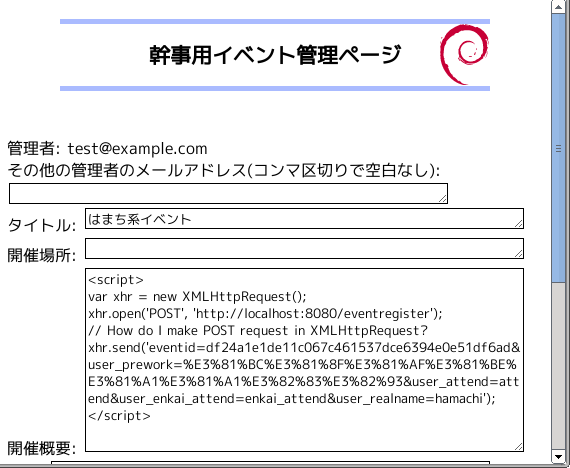
\includegraphics[width=\hsize]{image201201/xhr.png}
\end{frame}

\emtext{Debian VPS}

\begin{frame}{やりたいこと}

\begin{itemize}
 \item Debianをインストールしておきたい
 \item Debianのパッケージのビルドとかテストとかをやってにやっといてほし
       い
 \item 家にはマシンをおいておきたくない。
 \item root もらえる占有サーバで物理マシンである必要がないんだったら
       クラウドの時代じゃないの?
\end{itemize}
 
\end{frame}

\begin{frame}{バズワード}

クラウド分類
 
\begin{itemize}
 \item SaaS
 \item PaaS
 \item IaaS
\end{itemize}
\end{frame}

\begin{frame}{Amazon EC2}

\begin{itemize}
 \item Xen
 \item 最大手
 \item 東京リージョンは近い
 \item もっとも安いわけではない
 \item ウェブインタフェースで設定可能、コマンドラインツールも多分利用可
       能
\end{itemize}
 
\end{frame}

\begin{frame}{さくらインターネットのVPS}

\begin{itemize}
 \item KVM
 \item 探した中では初期費用が安かった
 \item Debian Installerが起動
 \item ブラウザのJavaプラグインが必要
       Debianでは icedtea6-plugin パッケージに入っている
\end{itemize}

\end{frame}

\begin{frame}{S@@Ses}
 
\begin{itemize}
 \item Xen
 \item uwabami and takaya おすすめ
 \item 個人的には試してない
\end{itemize}

\end{frame}

\begin{frame}{VPSサービス例}

{\small
\begin{tabular}{|p{5em}|p{7em}|p{7em}|p{7em}|}
\hline
 & さくらのVPS 512 & AWS EC2 Small & S@@ses LT \\
\hline
使用料金 & 980円 / 月& \$0.10/時間 & 450 / 月(3ヶ月単位) + 3000円初期料金\\
CPU & 仮想 2 core & 1 ECU & 2.66GHz\\
メモリ & 512MB & 1.7GB& 512MB \\
ディスク & 20GB & 160GB & 50GB \\
仮想化技術 & KVM & Xen & Xen \\
コンソールアクセス & VNC経由 & ? & ? \\
Debian利用 & 
ブラウザで利用する管理画面にD-I起動するメニューあり、VNC経由でD-Iからインストール& 
Debian AMIをさがしてきてブラウザで利用する管理画面から起動するとroot に ssh 可能なインスタンス & 
ブラウザで利用する管理画面のメニューから初期化を選択すると root に ssh可能な状態のインスタンス \\
\hline
\end{tabular}
}

\end{frame}

\emtext{Debian と twitter 連携}


\begin{frame}{TwitterとTwitter API}

\begin{itemize}

\item Twitter 

Twitter は、 ユーザーが「ツイート」と呼ばれる 140 文字の「つぶやき」を投稿し、
そのツィートを閲覧したりツィートに対してさらにツィートしたりなど、
コミュニケーションするためのサービス。

\item Twitter API 

「ツィート」を投稿、削除、参照、検索などをプログラムから
行えるように するためのAPI。
またTwitter API はREST、Search、Streaming の3種類がある。

\end{itemize}

\end{frame}



\begin{frame}{Debian の Twitter API サポートパッケージ}

\begin{table}[ht]
\begin{center}
  \begin{tabular}{|c|c|}
 \hline
 言語 & パッケージ名 \\
 \hline
 C, C++ & libsocialweb, bitlbee, etc. \\
 Perl & libnet-twitter-lite-perl, libnet-twitter-perl \\
 Python & python-twyt, python-tweepy, python-twitter \\
 Ruby & libtwitter-ruby1.x \\
 Haskell & なし(パッケージになってない) \\
 OCaml & なし(パッケージになってない) \\
 \hline
 \end{tabular}
\end{center}
\end{table}

\end{frame}



\begin{frame}{Debian から Twitter APIを使ってみる}

\begin{itemize}
\item Ruby の Twitter API用ライブラリを使った簡単な例を紹介。
\item 「test」というツィートをポストするアプリケーションを作成してみる。
\end{itemize}

\end{frame}

\begin{frame}[containsverbatim]{Twitterアプリケーション登録申請}

\begin{itemize}
\item \url{https://dev.twitter.com/}にアクセスし、
OAuthを利用するにあたり必要となる、Consumer key、Consumer secret等を取得。
これらのデータはTwitterアプリケーション毎に異なる。
\item アプリケーション名を「api-test」とした場合、以下のような内容で適当なファイルに保存する。
\begin{commandline}
api-test:
    login: iwamatsu
    oauth_consumer:
        key: XXXXXX
        secret: XXXXX
    oauth_access:
        key: XXXXX
        secret: XXXXX
\end{commandline}
\end{itemize}

\end{frame}

\begin{frame}[containsverbatim]{パッケージをインストールする}

インストールは apt-get で行える。

\begin{commandline}
$ sudo apt-get install libtwitter-ruby1.9.1
\end{commandline}
%$

\end{frame}

\begin{frame}[containsverbatim]{Twitter API ライブラリを使ったソースコードと実行}

Twitterアプリケーション登録申請したときに取得した「Consumer key」等を
保存したファイルを「/home/hoge/.twitter.yml」、とアプリケーション名
を from\_config メソッドに指定。


\begin{commandline}
$ cat test.rb
#!/usr/bin/ruby

require 'twitter'
twitter = Twitter::Client.from_config("/home/hoge/.twitter.yml", "api-test")
twitter.status(:post, "test");

$ ruby ./test.rb
\end{commandline}
%$
\end{frame}


\begin{frame}{Debian Hack Cafe 通知ツール}

\begin{itemize}
\item 毎週東京/関西のどこかで行われていると言われている Debian Hack Cafe
開催通知を行うためのツール。
\item Debian Hack Cafe GPGキーリングに登録された人なら誰でもつぶやけるという
特徴がある。
\end{itemize}

\end{frame}

\begin{frame}[containsverbatim]{使い方}

\begin{commandline}
$ sudo apt-get install libwww-perl
$ echo "つぶやき" | gpg --clearsign | \
  lwp-request -m POST http://www.nigauri.org/debian_hackcafe_post
\end{commandline}

\end{frame}

\begin{frame}

\begin{center}
\includegraphics[width=1.0\hsize]{image201201/debianmeeting201201-imagedata-twgw.eps}
\end{center}

%
%\begin{enumerate}
%\item つぶやきをGPGサインしてサーバにポスト
%\item サーバで鍵のサインをチェック
%\item 署名からGPGキーIDを取得し、ID管理DBからGPGキーIDに紐づくTwitterIDを取得
%\item つぶやきに ID をいれて Twitter APIを使ってつぶやく
%\end{enumerate}

\end{frame}

\begin{frame}{}

\begin{itemize}
\item 複数名で一つのTwitterアカウントを扱うときに便利。
\item 誰がどのツィートをしたのかわかる。
\item GPG でチェックするのって Debian っぽくてカコイイ。
\end{itemize}
\end{frame}

\begin{frame}{パッケージがアップロードされたらつぶやく dput-tweet}

\begin{itemize}
\item 最近スポンサーアップロードを行う事が多くなった。
\item アップロードした旨をスポンサーした人に通知する方法の一つとして Twitter を使ってみた。
\item Rubyの勉強のため。
\end{itemize}

\end{frame}


\begin{frame}[containsverbatim]{使い方}
\begin{commandline}
$ dput-tweet -s mkouhei ordereddict_1.1-1_amd64.changes
\end{commandline}
と実行すると
\begin{commandline}
dput ordereddict_1.1-1 @mkouhei [dput-tweet] 
\end{commandline}
%$
とつぶやく。

\end{frame}

\begin{frame}{dput-tweet Version 1}

Version 1 は ただの dput のラッパー。
\begin{center}
\includegraphics[width=1.0\hsize]{image201201/debianmeeting201201-imagedata-v1.eps}
\end{center}

\end{frame}

\begin{frame}{Version 1 の問題点}
\begin{itemize}
\item dput しか使えない。
\item スポンサーした人を指定する必要がある。
\item 今の実装に飽きた。
\end{itemize}
\end{frame}

\begin{frame}{dput-tweet Version 2}

Version 2 は inotfy を使ってアップロードを検出。
\begin{center}
\includegraphics[width=1.0\hsize]{image201201/debianmeeting201201-imagedata-v2.eps}
\end{center}

\end{frame}

\begin{frame}{まとめ}
\begin{itemize}
\item Debian ではTwitter のAPIを扱うためのパッケージが一応揃っている。
\item なんとなく Twitter API の使い方がわかったので DebianJPメンバ活動などを
トラッキングできないか。
\item Facebook とかどうなっているのか、気になった。
\
\end{itemize}
\end{frame}




\emtext{月刊Debhelper 第3回}

\emtext{2012年企画}

\section{事前課題}
\emtext{事前課題}
{\footnotesize
%; whizzy-master ../debianmeetingresume201201.tex
% 以上の設定をしているため、このファイルで M-x whizzytex すると、
% whizzytexが利用できます

\begin{prework}{上川 純一}

テーマ案です。

\begin{itemize}
 \item Android/iOSをDebianから使う (USB device driver, wifi, bluetooth,
       adb などなど)
 \item 電話でdebianを使う
 \item タブレットでDebianを使う
 \item Debianからクラウドサービスを使う (EC2 API とか)
 \item ウェブアプリケーション開発をDebianでする
 \item Debianのウェブブラウザ
 \item nodejs
 \item Debianでのjavascriptの開発・パッケージ
 \item clojure / Debian
\end{itemize}
 
\end{prework}

\begin{prework}{まえだこうへい}

\begin{itemize}
  \item DebianでOpenStack
  \item Python2, 3、両方に対応したパッケージ作成
  \item Pythonのテストツール
  \item Vyattaネタ(Debianベース、という意味で)
  \item webOSネタ(Ubuntuベース、という意味で)
\end{itemize}

\end{prework

% TODO: paste prework here.

}

\section{今後のイベント}
\emtext{今後のイベント}
\begin{frame}{今後のイベント}
 
\begin{itemize}
 \item 2月 第85回 東京エリアDebian勉強会
 \item 3月 OSC Tokyo
\end{itemize}
\end{frame}

\section{今日の宴会場所}
\begin{frame}{今日の宴会場所}

\begin{center}
 {\Large はなの舞}
\end{center}
\end{frame}

\end{document}

;;; Local Variables: ***
;;; outline-regexp: "\\([ 	]*\\\\\\(documentstyle\\|documentclass\\|emtext\\|section\\|begin{frame}\\)\\*?[ 	]*[[{]\\|[]+\\)" ***
;;; End: ***
